\chapter{Experiments and Results}\label{cpt:exp}

\section{Implementation Settings}

Donec porttitor tempor dui, ut aliquet dui ultrices sed. Nunc malesuada in Fig.\ref{fig:result1}, tellus quis efficitur dignissim, ante dui viverra diam, sit amet porta velit est vitae quam. Sed odio elit, sagittis a tellus id, rhoncus maximus augue. Donec consectetur nisi sit amet ante venenatis dictum. Nam sit amet cursus augue, quis maximus lacus. Nulla rhoncus egestas erat, vel consectetur nisl ornare ac. Pellentesque habitant morbi tristique senectus et netus et malesuada fames ac turpis egestas. Fusce rutrum imperdiet hendrerit. Aenean eu lobortis metus. Vestibulum fermentum, lacus nec euismod viverra, enim sem auctor turpis, eget tincidunt nisl augue sed elit.

\figpdf{Experimental result 1}{result1}{11cm}

\section{Result 1}

Aenean ultrices felis ante, in neque dictum ut. Class aptent taciti sociosqu ad litora torquent per conubia nostra, per inceptos himenaeos. Vestibulum ante ipsum primis in faucibus orci luctus et ultrices posuere cubilia Curae; Maecenas porta ex quis erat egestas condimentum. Donec suscipit semper egestas. Vestibulum id massa aliquet, ullamcorper nibh vel, porttitor leo. Cras porta leo et diam tincidunt, ut viverra metus varius \Fig{result2}.

\figpdf{Experimental result 2}{result2}{9cm}

\section{Result 2}

In Fig.\ref{fig:result2}, curabitur consequat sodales ligula in condimentum. Praesent imperdiet, nulla eu egestas ultrices, diam elit fringilla purus, sit amet elementum lacus mauris vitae turpis. Nunc lobortis viverra est, vel porttitor orci eleifend ac. Vestibulum lacus ante, finibus a est id, ornare viverra orci. Pellentesque habitant morbi tristique senectus et netus et malesuada fames ac turpis egestas. Nam ultricies, ligula a ultrices eleifend, mi lectus interdum leo, sit amet fringilla nisi odio sit amet lectus. Nam cursus eros a mi vestibulum, sit amet lobortis lacus consectetur.



\begin{figure}[htp] %htp用来表示图片的位置
\centering 
  \subfigure[Description 1]{ 
    \label{fig:subfig:a} % 第1幅图的的标签
    % 第1幅图片的尺寸和地址
    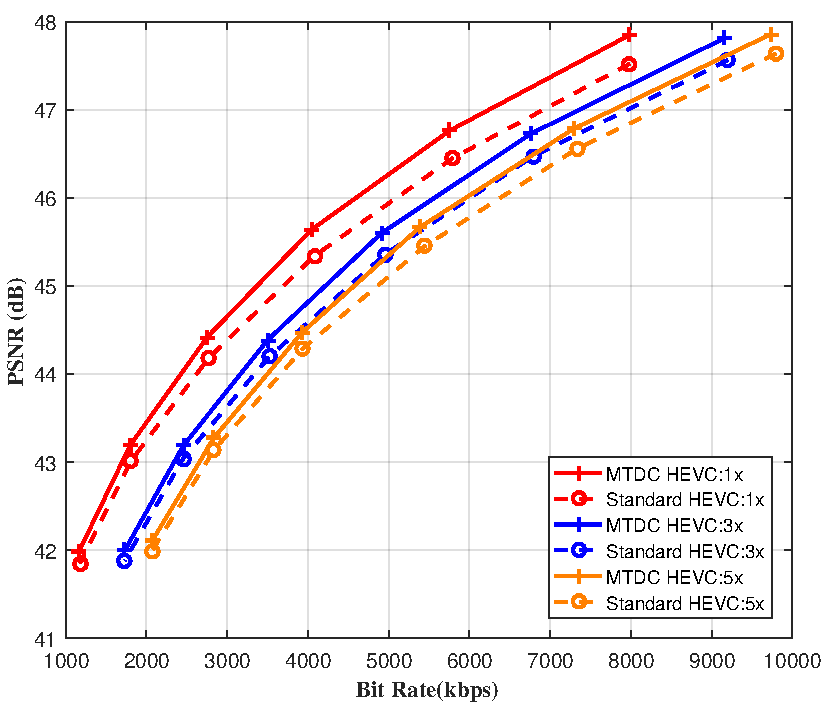
\includegraphics[width=6cm]{fig/sub1.pdf}}
  \hspace{0.5cm} % 图片的水平间隔
  \subfigure[Description 2]{ 
    \label{fig:subfig:b} % 第2幅图的的标签 
    % 第1幅图片的尺寸和地址
    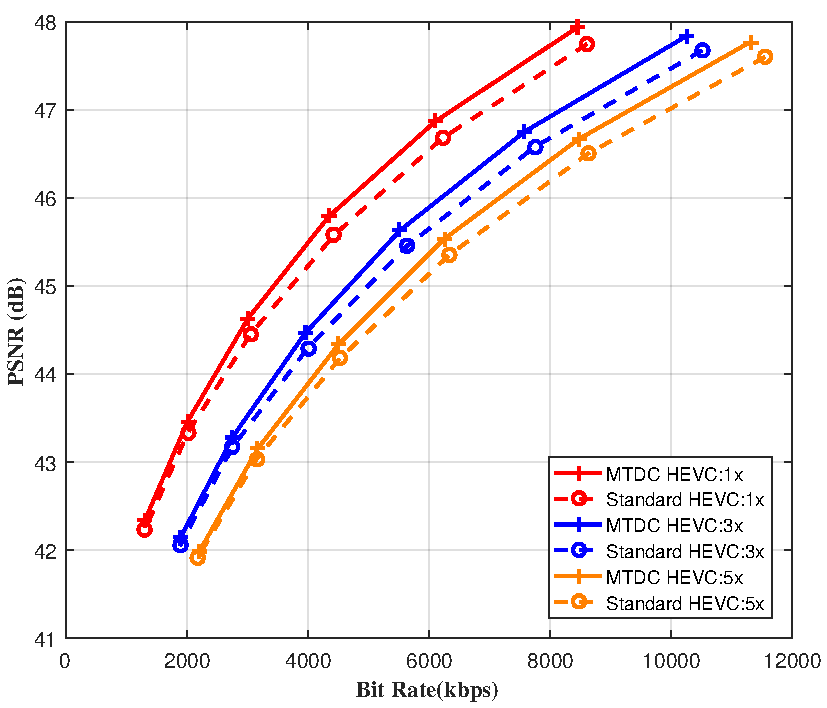
\includegraphics[width=6cm]{fig/sub2.pdf}} 
  \\ % 强制换行
  \vspace{0.5cm} % 图片的垂直间隔
  \subfigure[Description 3]{ 
    \label{fig:subfig:c} % 第3幅图的的标签
    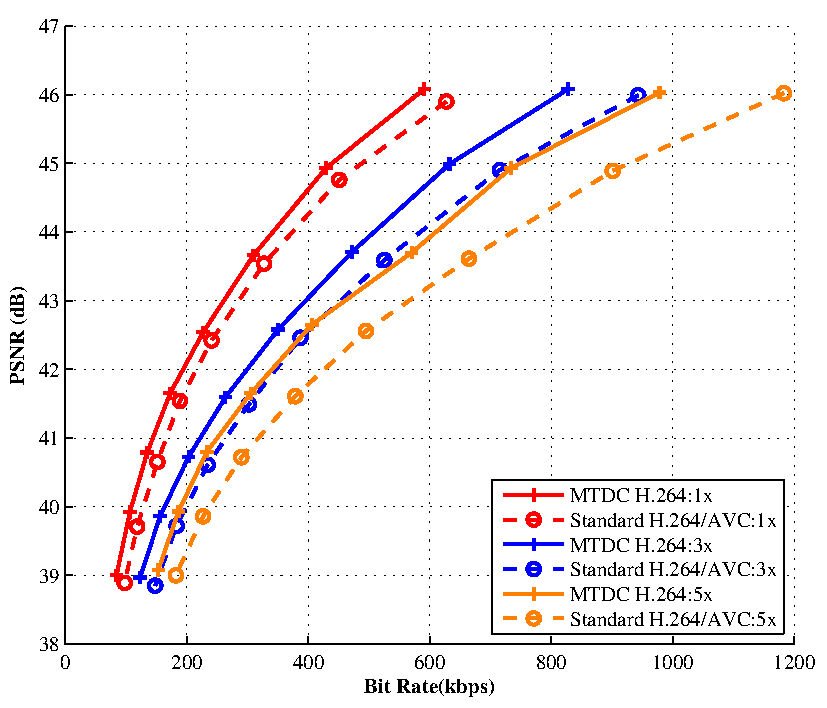
\includegraphics[width=6cm]{fig/sub3.pdf}} 
  \hspace{0.5cm} % 图片的水平间隔
  \subfigure[Description 4]{ 
    \label{fig:subfig:d} % 第4幅图的的标签
    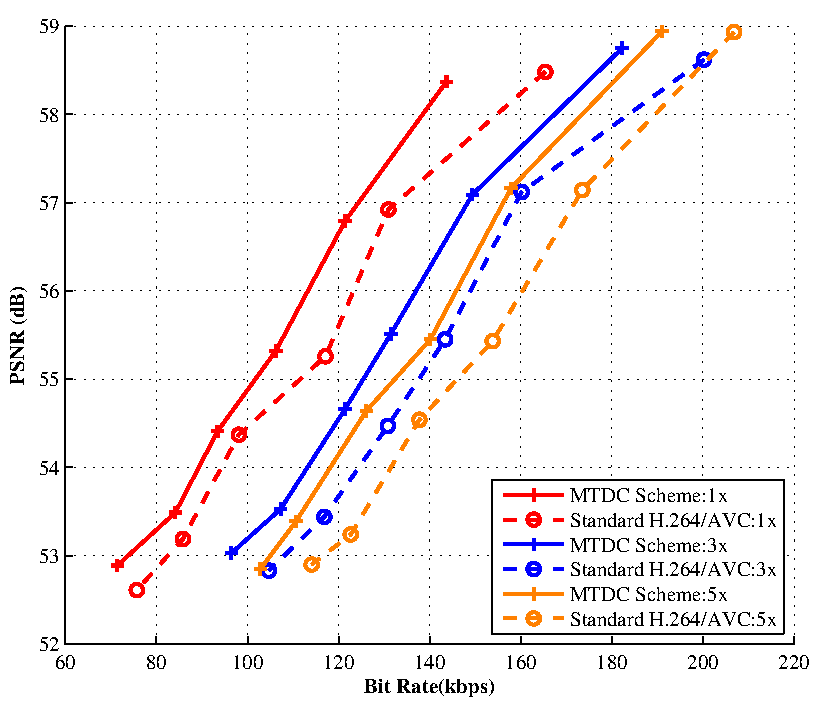
\includegraphics[width=6cm]{fig/sub4.pdf}} 
  \caption{For sub firgures located in a $2\times 2$ array} 
  \label{fig:subfig} %% label for entire figure 
\end{figure}

\begin{table}[h]
\label{tab:tab2}
\centering
\caption{ Title Of Table }
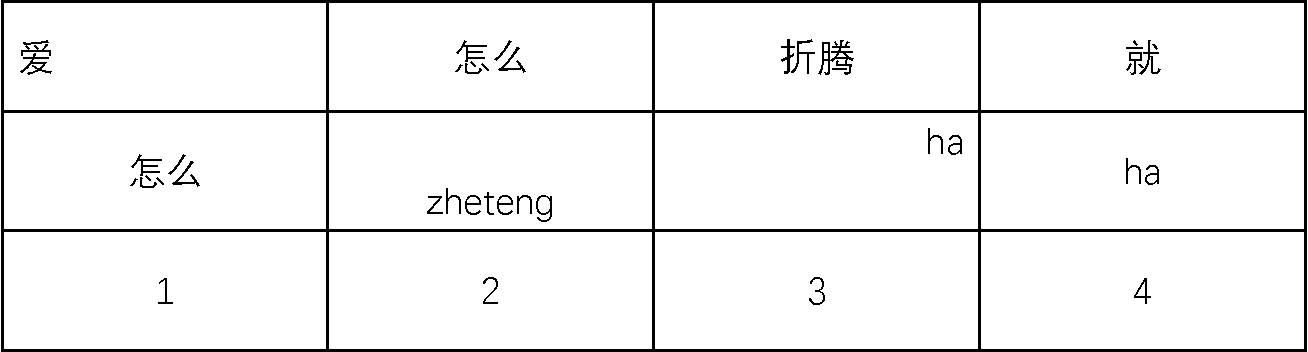
\includegraphics[width=10cm]{fig/table.pdf}
\end{table}

Sed at leo eleifend ante dapibus sollicitudin. Donec eget turpis massa. Fusce efficitur, sem eu sollicitudin rhoncus, eros nulla aliquet arcu, ut pellentesque lacus metus eu turpis. Duis venenatis eleifend leo, non lobortis tortor dictum sed. Cras eu dui quis dolor scelerisque eleifend sit amet a nibh. Suspendisse porttitor sit amet nunc sit amet hendrerit. Fusce tempus purus metus, rhoncus dictum nisl pretium vitae. Suspendisse sodales nunc velit, ac malesuada diam commodo sed. Sed maximus vel risus quis laoreet. Ut ullamcorper ante non faucibus imperdiet. Cras tristique nec ligula id egestas. Duis ut elit id lorem sodales viverra eu ut leo in Equ.\ref{equ:equation1}.

\begin{equation}\label{equ:equation1}
R^m_T=R_{180\Omega}+R_{100\Omega}+R_{120\Omega}
\end{equation}

%见到的令你感动的代码插入功能,将c代码加入到
%\code{c++}{c_test.c}
